\chapter{Исследовательская часть}

\section{Технические характеристики}

Технические характеристики устройства, на котором выполнялись замеры по времени:

\begin{itemize}
	\item Процессор: Apple M1 Pro \cite{m1}
	\item Оперативная память: 32 ГБайт.
	\item Операционная система: macOS Ventura 13.5.2. \cite{macOS}
\end{itemize}

При замерах времени ноутбук был включен в сеть электропитания и был нагружен только системными приложениями.

\section{Демонстрация работы программы}

На изображении \ref{img:example} представлена иллюстрация работы разработанного программного продукта. 
Конкретно, демонстрируются результаты выполнения алгоритмов поиска подстроки в строке
\clearpage
\begin{figure}[h]
	\centering
	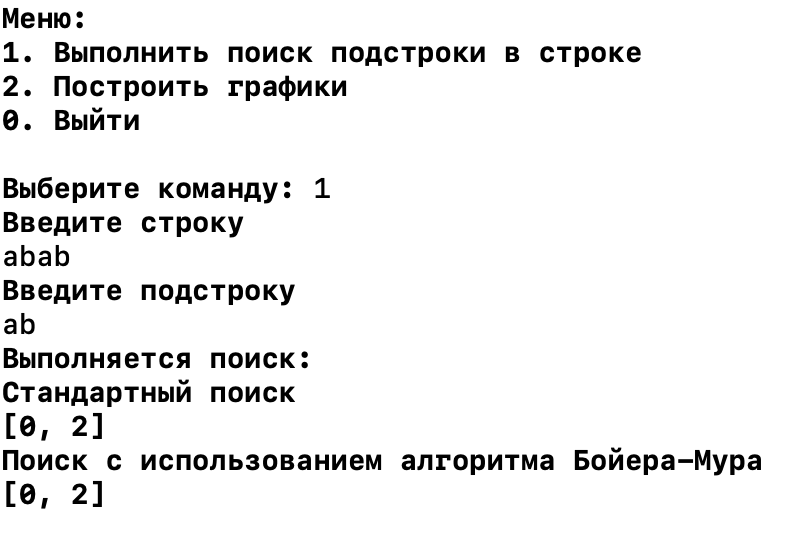
\includegraphics[height=0.3\textheight]{img/example.png}
	\caption{Демонстрация работы программы}
	\label{img:example}
\end{figure}

\clearpage
\section{Анализ временных характеристик}

В данном разделе представлены результаты экспериментов, в которых измерялось время выполнения поиска подстроки в строке в лучшем случае, худшем случае и на случайных данных, где лучший случай -- нахождение подстроки в строке на первой позиции, худший -- отстутствие подстроки в строке. 
Данные результаты представлены в таблицах \ref{tbl:time_table_best} -- \ref{tbl:time_table_avg}.

Таблица \ref{tbl:time_table_best} содержит результаты замеров времени выполнения алгоритмов поиска подстроки в строке для строк, являющихся шестнадцатеричным кодом длинами $2^8$, $2^{10}$, $2^{12}$, $2^{14}$, $2^{16}$ в лучшем случае.

\begin{table}[ht]
	\small
	\begin{center}
		\begin{threeparttable}
		\caption{Результаты замеров времени, лучший случай}
		\label{tbl:time_table_best}
		\begin{tabular}{|c|c|c|}
			\hline
			& \multicolumn{2}{c|}{\bfseries Время, мкс} \\ \cline{2-3}
			\bfseries Длина строки & \bfseries Стандартный & \bfseries Бойера~---~Мура
			\csvreader{csv/data_best.csv}{} 
			{\\\hline \csvcoli & \csvcolii & \csvcoliii} \\
			\hline
		\end{tabular}	
		\end{threeparttable}
	\end{center}
\end{table}

На основе данных из таблицы \ref{tbl:time_table_best} был построен график (см. рисунок \ref{plt:graph_best}).
\clearpage

\begin{figure}[h]
	\centering
	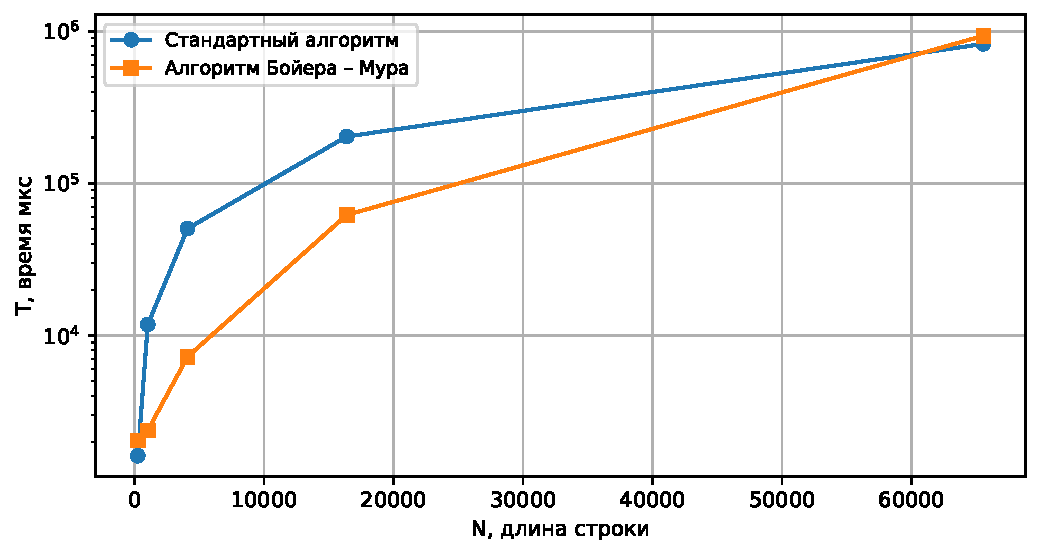
\includegraphics[height=0.3\textheight]{img/graph_best.pdf}
	\caption{Сравнение времени выполнения алгоритмов поиска подстроки в строке, лучший случай}
	\label{plt:graph_best}
\end{figure}

Таблица \ref{tbl:time_table_worst} содержит результаты замеров времени выполнения алгоритмов поиска подстроки в строке для строк, являющихся шестнадцатеричным кодом длинами $2^8$, $2^{10}$, $2^{12}$, $2^{14}$, $2^{16}$ в худшем случае.

\begin{table}[ht]
	\small
	\begin{center}
		\begin{threeparttable}
		\caption{Результаты замеров времени, худший случай}
		\label{tbl:time_table_worst}
		\begin{tabular}{|c|c|c|}
			\hline
			& \multicolumn{2}{c|}{\bfseries Время, мкс} \\ \cline{2-3}
			\bfseries Длина строки & \bfseries Стандартный & \bfseries Бойера~---~Мура
			\csvreader{csv/data_worst.csv}{} 
			{\\\hline \csvcoli & \csvcolii & \csvcoliii} \\
			\hline
		\end{tabular}	
		\end{threeparttable}
	\end{center}
\end{table}

На основе данных из таблицы \ref{tbl:time_table_worst} был построен график (см. рисунок \ref{plt:graph_worst}).
\clearpage

\begin{figure}[h]
	\centering
	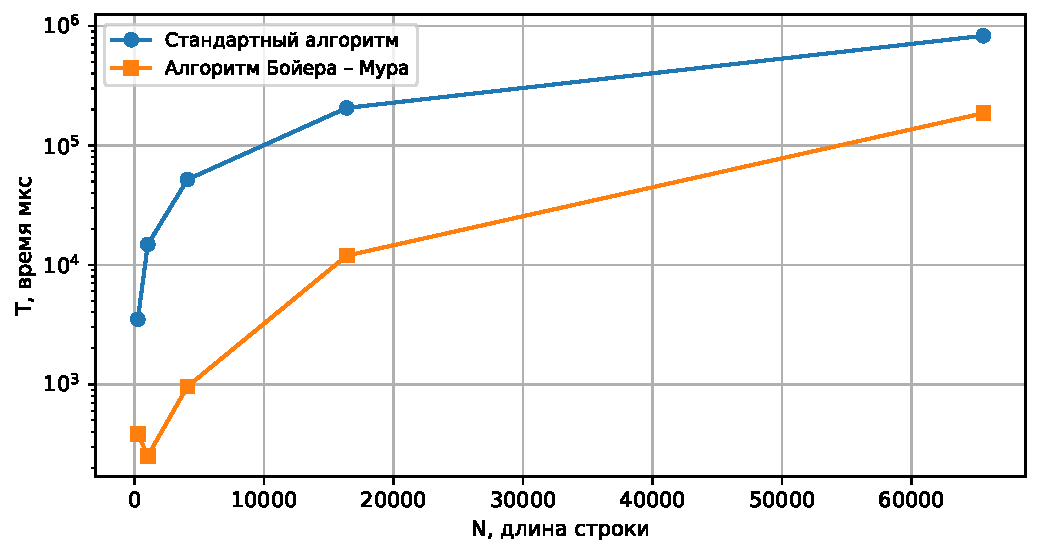
\includegraphics[height=0.3\textheight]{img/graph_worst.pdf}
	\caption{Сравнение времени выполнения алгоритмов поиска подстроки в строке, худший случай}
	\label{plt:graph_worst}
\end{figure}

Таблица \ref{tbl:time_table_avg} содержит результаты замеров времени выполнения алгоритмов поиска подстроки в строке для строк, являющихся шестнадцатеричным кодом длинами $2^8$, $2^{10}$, $2^{12}$, $2^{14}$, $2^{16}$ на случайном наборе данных.

\begin{table}[ht]
	\small
	\begin{center}
		\begin{threeparttable}
		\caption{Результаты замеров времени, случайные данные}
		\label{tbl:time_table_avg}
		\begin{tabular}{|c|c|c|}
			\hline
			& \multicolumn{2}{c|}{\bfseries Время, мкс} \\ \cline{2-3}
			\bfseries Длина строки & \bfseries Стандартный & \bfseries Бойера~---~Мура
			\csvreader{csv/data_avg.csv}{} 
			{\\\hline \csvcoli & \csvcolii & \csvcoliii} \\
			\hline
		\end{tabular}	
		\end{threeparttable}
	\end{center}
\end{table}

На основе данных из таблицы \ref{tbl:time_table_avg} был построен график (см. рисунок \ref{plt:graph_avg}).
\clearpage

\begin{figure}[h]
	\centering
	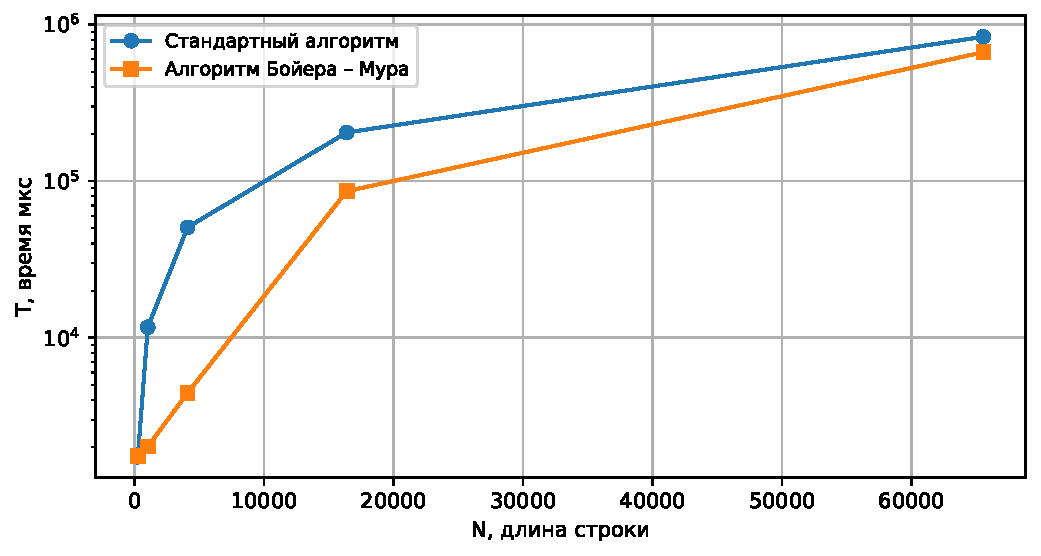
\includegraphics[height=0.3\textheight]{img/graph_avg.pdf}
	\caption{Сравнение времени выполнения алгоритмов поиска подстроки в строке, случайный набор данных}
	\label{plt:graph_avg}
\end{figure}

\section{Выводы}
Результаты экспериментов позволяют сделать вывод о том, что в лучшем случае реализация алгоритма Бойера~--~Мура менее эффективна по времени стандартного алгоритма, начиная с размера строки $2^{16}$.
Наилучшие показатели реализация алгоритма Бойера~--~Мура показывает в худшем случае -- она может быть эффективнее стандартного алгоритма вплоть до 10 раз.